
\begin{frame}
  \begin{columns}
    \begin{column}{.8\textwidth}
      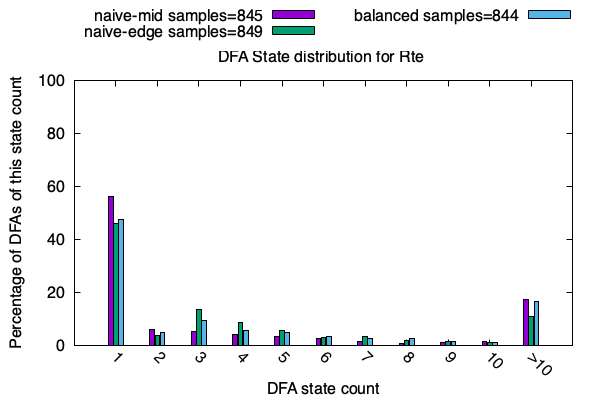
\includegraphics[width=0.9\textwidth, height=0.9\textheight, keepaspectratio]{plot-histogram.png}      
    \end{column}
    \begin{column}{.33\textwidth}
      Balanced sampling results in $\approx 24$ to 26\% of DFAs with 10 states or larger.
      Tree-split (uneven) results in $\approx 27\%$.
      Worst performing is the comb distribution.
    \end{column}
  \end{columns}
\end{frame}



\begin{frame}
  \begin{columns}
    \begin{column}{.8\textwidth}
      \includegraphics[width=0.9\textwidth, height=0.9\textheight, keepaspectratio]{plot-64-histogram.png}      
    \end{column}
    \begin{column}{.33\textwidth}
      \textcolor{orange}{Restricted to RTEs with exactly 64 leaf nodes.}

      \medskip

      Balanced sampling results in $\approx 22$ to 23\% of DFAs with 10 states or larger.
      Uniform sampling results in in range $20 \%$ to 23.
    \end{column}
  \end{columns}

\end{frame}

\begin{frame}
  \begin{columns}
    \begin{column}{.8\textwidth}
      \includegraphics[width=0.9\textwidth, height=0.9\textheight, keepaspectratio]{plot-128-histogram.png}      
    \end{column}
    \begin{column}{.33\textwidth}
      \textcolor{orange}{Restricted to larger RTEs with exactly 128 leaf nodes.}

      \medskip

      Balanced sampling results in $\approx 20\%$ to 32 of DFAs with 10 states or larger.


      \medskip

      Imbalanced, results in $< 5\%$ 
    \end{column}
  \end{columns}
\end{frame}


\begin{frame}{How to measure aspect-ratio of a binary tree}

  \emph{CLAIM}: a \emph{Landscape-style} AST performs better than \emph{Portrait-style}.


  \scalebox{1.1}{\input{aspect-ratio}}
  \vspace{-8mm}
  \begin{columns}
    \begin{column}{0.5\textwidth}
      \[\rho = \text{aspect ratio} = \frac{d}{\log_2 n} = \frac{\text{longest path}}{\log_2(\text{leaf count})}\]      
    \end{column}
    \begin{column}{0.5\textwidth}
    \begin{align*}
      \rho = 1 & \implies \text{balanced}\\
      \rho < 1 & \implies \text{landscape}\\
      \rho > 1 & \implies \text{portrait}
    \end{align*}
    \end{column}
  \end{columns}

\end{frame}




% use this box via:    \usebox\arbox
\newsavebox\arbox
\begin{lrbox}{\arbox}
  \begin{minipage}{4cm}
    \[\rho = \frac{longest~path}{\log_2(leaf~count)}\]

    \begin{align*}
      \rho = 1 & \implies \text{balanced}\\
      \rho < 1 & \implies \text{landscape}\\
      \rho > 1 & \implies \text{portrait}
    \end{align*}
  \end{minipage}
\end{lrbox}

\begin{frame}
  \begin{columns}
    \begin{column}{.8\textwidth}
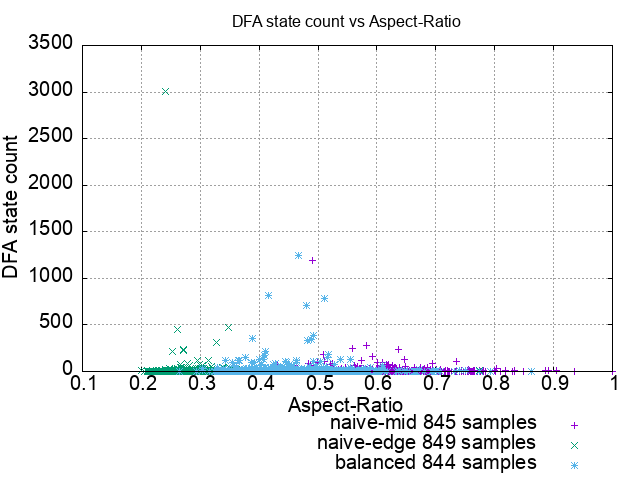
\includegraphics[width=0.9\textwidth, height=0.9\textheight, keepaspectratio]{plot-dfa-state-count-vs-Aspect-Ratio.png}
    \end{column}
    \begin{column}{.35\textwidth}
      DFA state count \\vs Aspect Ratio

      \usebox\arbox
    \end{column}
  \end{columns}
\end{frame}

\begin{frame}
  \begin{columns}
    \begin{column}{.8\textwidth}
\includegraphics[width=0.9\textwidth, height=0.9\textheight, keepaspectratio]{plot-dfa-state-count-vs-Aspect-Ratio-ratsnest.png}
    \end{column}
    \begin{column}{.35\textwidth}
      DFA state count \\vs Aspect Ratio

      \usebox\arbox
    \end{column}
  \end{columns}
\end{frame}



\begin{frame}
  \begin{columns}
    \begin{column}{.8\textwidth}
\includegraphics[width=0.9\textwidth, height=0.9\textheight, keepaspectratio]{plot-64-dfa-state-count-vs-Aspect-Ratio-ratsnest.png}
    \end{column}
    \begin{column}{.35\textwidth}
      \textcolor{orange}{Restricted to RTEs having exactly 64 leaf nodes.}

      \medskip
      
      DFA state count \\vs Aspect Ratio

      \usebox\arbox
    \end{column}
  \end{columns}
\end{frame}

\begin{frame}
  \begin{columns}
    \begin{column}{.8\textwidth}
\includegraphics[width=0.9\textwidth, height=0.9\textheight, keepaspectratio]{plot-128-dfa-state-count-vs-Aspect-Ratio-ratsnest.png}
    \end{column}
    \begin{column}{.35\textwidth}
      \textcolor{orange}{Restricted to RTEs having exactly 128 leaf nodes.}

      \medskip
      

      DFA state count \\vs Aspect Ratio

      \usebox\arbox
    \end{column}
  \end{columns}
\end{frame}






\begin{frame}
  \begin{columns}
    \begin{column}{.8\textwidth}
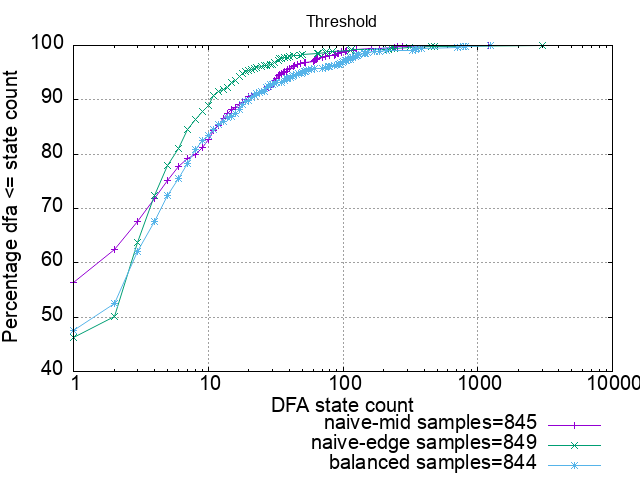
\includegraphics[width=0.9\textwidth, height=0.9\textheight, keepaspectratio]{plot-threshold.png}
    \end{column}
    \begin{column}{.35\textwidth}
      Which percent of all DFAs have larger than x-many states?

      \medskip
      
      Flajolet and tree-split-mid (Gaussian) produces 10\% of DFAs larger than 50 states.

      Tree-split-edge (inverted Gaussian) and tree-split-linear produces 11\% larger than 10 states.

      Imbalanced produces 1\% larger than 11 states.
    \end{column}
  \end{columns}
\end{frame}




\begin{frame}
  \begin{columns}
    \begin{column}{.8\textwidth}
\includegraphics[width=0.9\textwidth, height=0.9\textheight, keepaspectratio]{plot-64-threshold.png}
    \end{column}
    \begin{column}{.33\textwidth}
      \textcolor{orange}{Restricted to RTEs with exactly 64 leaf nodes.}

    \end{column}
  \end{columns}
\end{frame}

\begin{frame}
  \begin{columns}
    \begin{column}{.8\textwidth}
\includegraphics[width=0.9\textwidth, height=0.9\textheight, keepaspectratio]{plot-128-threshold.png}
    \end{column}
    \begin{column}{.33\textwidth}
      \textcolor{orange}{Restricted to RTEs with exactly 128 leaf nodes.}

      \medskip

      There seems to be some convergence of behavior for all the somewhat balanced algorithms
      for large RTEs.

    \end{column}
  \end{columns}
\end{frame}

